\chapter{Higgs boson at the LHC: Phenomenology}
\label{sec:LHC_Pheno}
\chaptermark{Higgs boson at the LHC: Phenomenology}


In this section we discuss specific phenomenological details that are studied for this thesis. First, we discuss the different modes of producing a Higgs boson at the LHC, and different features of these different production modes. Next, we will present the decay of a Higgs boson decay to two Z bosons and subsequently four leptons. Using this information we will present the implications of off resonance production and decay on the Higgs lifetime. Finally, we will discuss the spin and parity of a single-produced resonance and how we can use these relations to characterize a new particle found at the LHC.

\section{Higgs boson production at LHC}
\label{sec:Higgs_Production_Pheno}

In proton-proton collisions a SM Higgs boson can be produced through the coupling of a Higgs boson to either bosons or fermions. Each of these two categories of Higgs production will be dominated by specific production modes. Fermionic production of a Higgs boson can happen either through \textit{gluon-gluon fusion} $gg \to H$ (ggH) and much less frequently through production in \textit{association with two top quarks} $gg \to H + t\bar{t}$ (ttH). Bosonic production of a Higgs boson can occur through \textit{vector boson fusion} (VBF), where two quarks radiate vector bosons which produce the boson in association with two quark jets $qq \to H + 2\text{jets}$ or through production \textit{associated with a vector boson} $qq \to H + W/Z$ (VH).

The cross sections of these different production mechanisms as a function of the Higgs boson mass at the LHC are shown in figure \ref{fig:LHC_Hxsec} for the two center of mass energies used in this thesis; $\sqrt{s} = \unit{7}{\TeV}$ and $\sqrt{s} = \unit{8}{\TeV}$ \cite{Dittmaier:2011ti, Dittmaier:2012vm}. Notable features of these cross sections are the order of magnitude difference between gluon-gluon fusion and the bosonic production modes which are all much larger than the $gg \to H + t\bar{t}$ production. Additionally, one can see the boost in the gluon-gluon fusion production at $2m_{t}$, which corresponds to the top quark in the production loop going becoming on shell (explained in more detail below).

\begin{figure}
\begin{center}
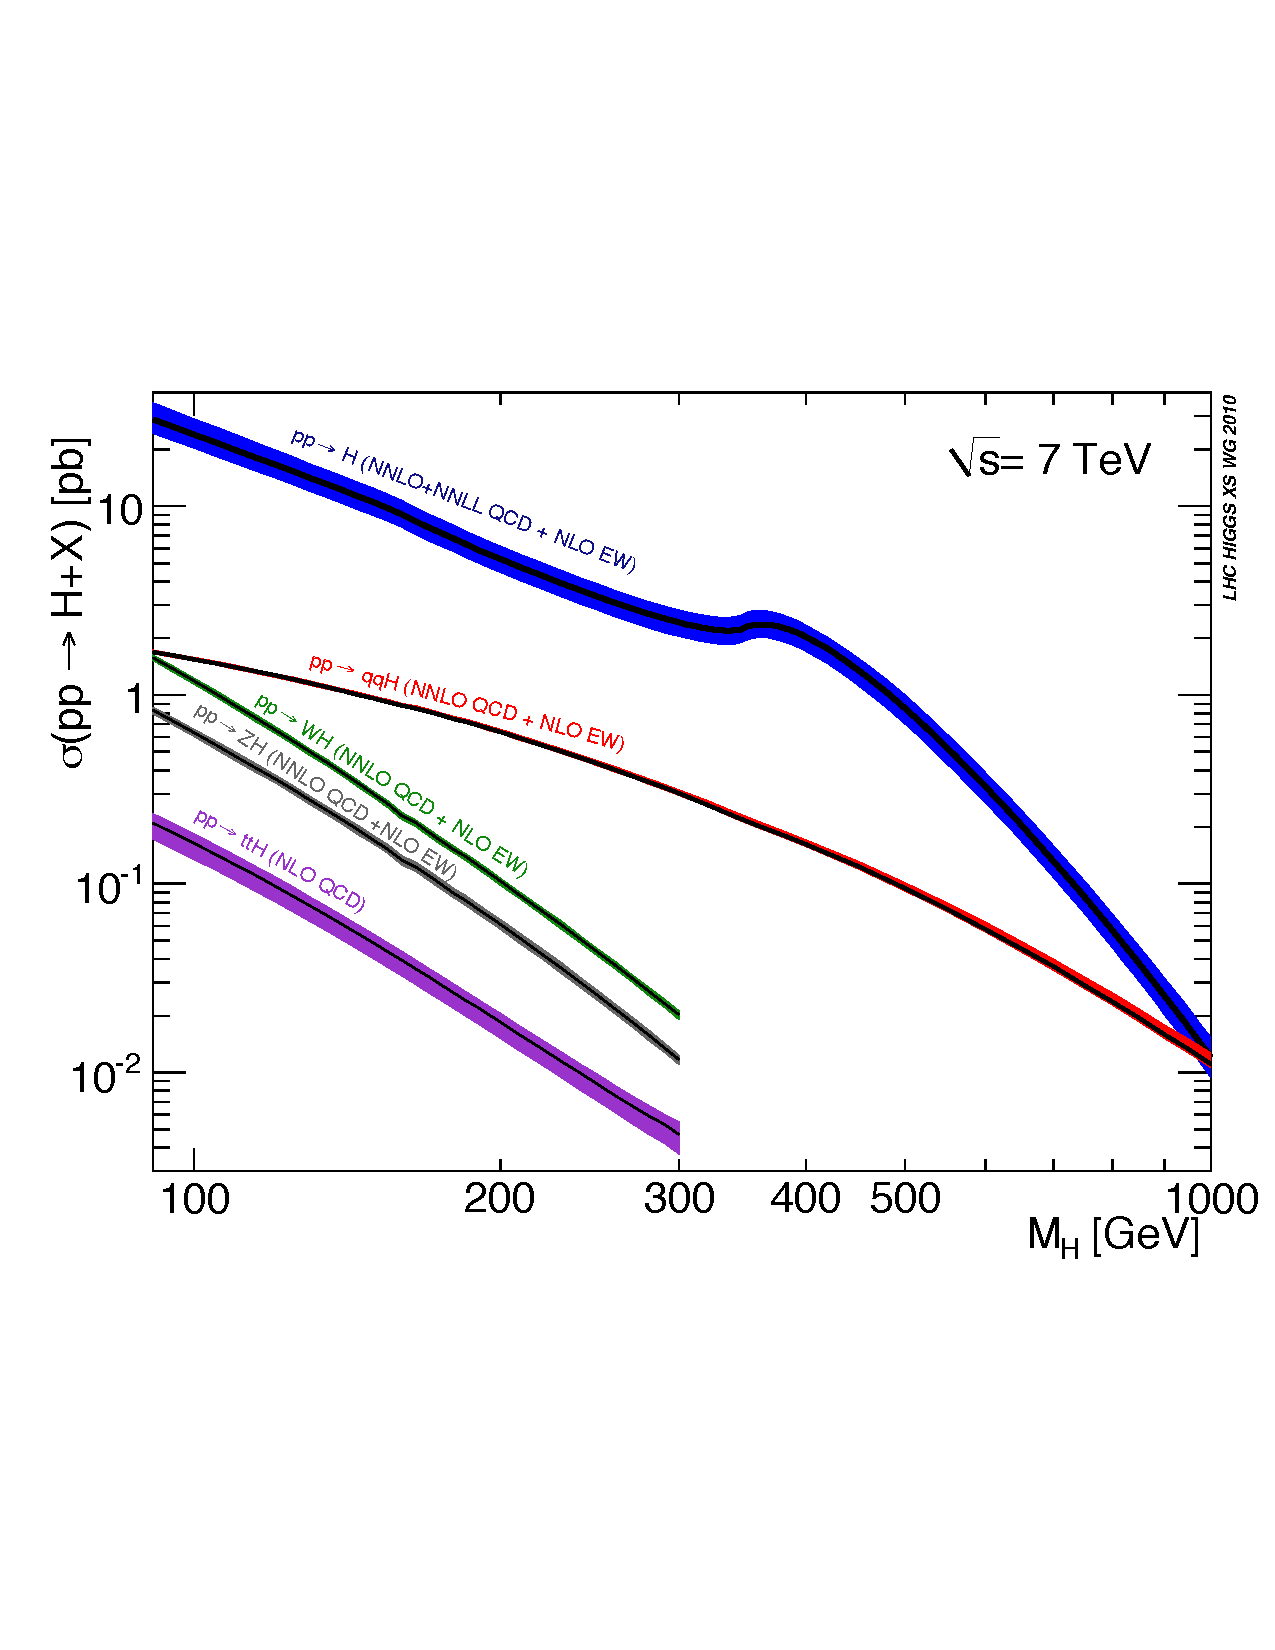
\includegraphics[width=0.46\linewidth]{{LHC_Pheno/Higgs_XS_7TeV}.pdf}
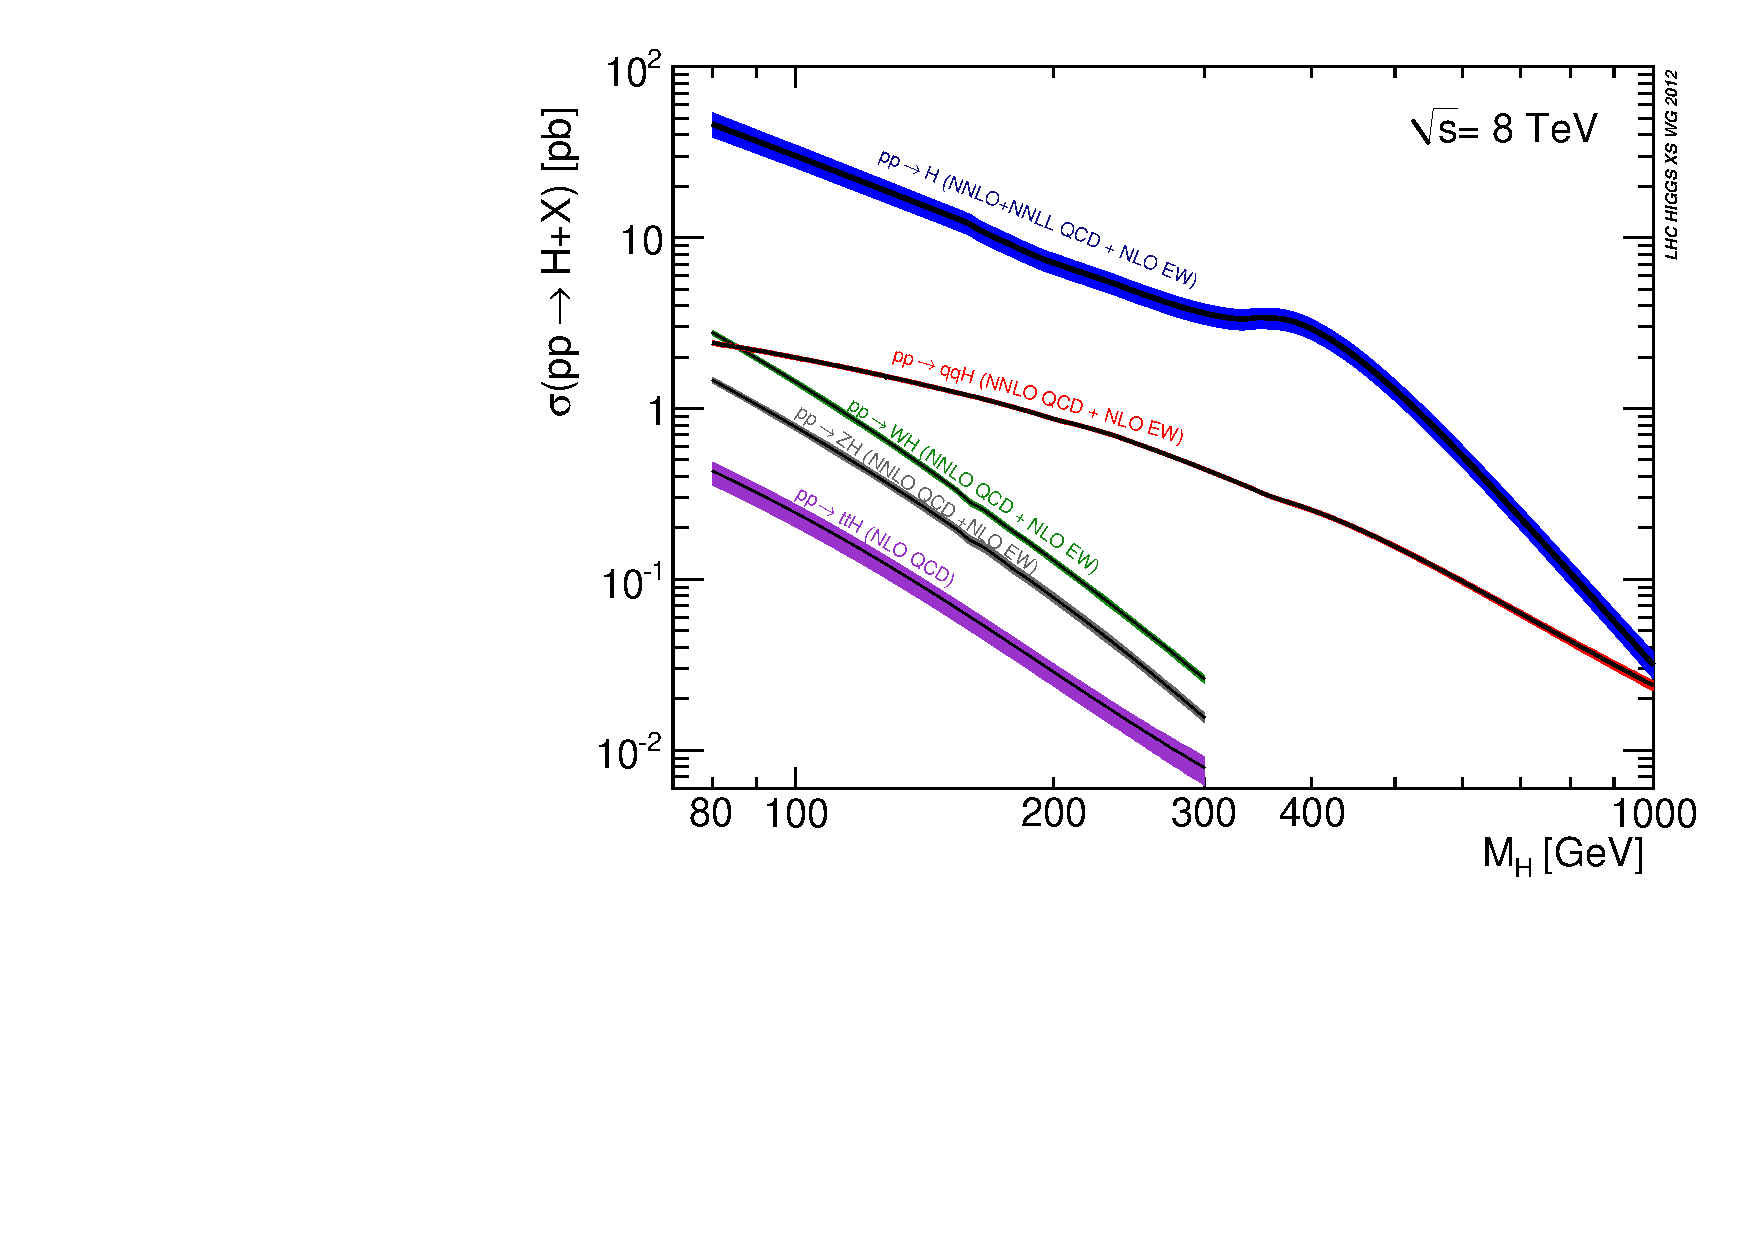
\includegraphics[width=0.455\linewidth]{{LHC_Pheno/Higgs_XS_8TeV_lx}.pdf}
\caption[Standard Model Higgs boson production cross sections and relative uncertainties at $\sqrt{s} = \unit{7}{\TeV}$ and $\sqrt{s} = \unit{8}{\TeV}$. From top to bottom these are $pp \to H$, blue, $pp \to H + 2\text{jets}$, red, $pp \to H + W$, green, $pp \to H + Z$, grey, $pp \to H + t\bar{t}$, purple.]{Standard Model Higgs boson production cross sections and relative uncertainties at $\sqrt{s} = \unit{7}{\TeV}$ and $\sqrt{s} = \unit{8}{\TeV}$. From top to bottom these are $pp \to H$, blue, $pp \to H + 2\text{jets}$, red, $pp \to H + W$, green, $pp \to H + Z$, grey, $pp \to H + t\bar{t}$, purple \cite{Dittmaier:2011ti, Dittmaier:2012vm}.}
\label{fig:LHC_Hxsec}
\end{center}
\end{figure}

The main production mechanism at the LHC is gluon-gluon fusion. The Feynman diagram for this process is shown in figure \ref{fig:ggH_Feyn}. While the Higgs boson does not couple directly to gluons (because they are massless) this mode of production relies on the Higgs coupling to fermions generated by the incoming gluons. Because the coupling of the Higgs is proportional to the mass of the fermion the dominant contribution is the Higgs -- top coupling. This leads to a boost in the cross section when the mass of the Higgs is twice the top mass because the top's in the loop are no longer virtual. For the entire mass range that is considered in this analysis this is the most common way to produce a Higgs boson at the LHC.

\begin{figure}
\begin{center}
\unitlength=1mm
\begin{fmffile}{ggH_Feyn}

\begin{fmfgraph*}(40,30) 
  \fmfleft{i1,i2} \fmfright{sp1}
  \fmf{gluon,label=$g$}{i1,v1} 
  \fmf{gluon,label=$g$}{i2,v2}
  \fmf{fermion}{v1,v2,v3,v1}
  \fmffixed{(0,.6h)}{v1,v2}
  \fmf{scalar,label=$H$}{v3,sp1}
\end{fmfgraph*}

\end{fmffile}
\end{center}
\caption[Feynman diagram depicting Higgs boson production through gluon-gluon fusion $gg \to H$. The fermion loop is dominated by top quarks, however all quarks contribute according to their masses.]{Feynman diagram depicting Higgs boson production through gluon-gluon fusion $gg \to H$. The fermion loop is dominated by top quarks, however all quarks contribute according to their masses.}
\label{fig:ggH_Feyn}
\end{figure}

The second most likely way to produce a Higgs at the LHC is through vector boson fusion. To produce a Higgs this way two quarks exchange a W or Z boson which radiates the Higgs boson. This production mode relies on the Higgs boson coupling to the vector bosons, making it distinct compared to gluon-gluon fusion. the distinguishing feature of this production mode is the presence of two quark jets in the final state in addition to the Higgs boson. These jets contain information about the Higgs and can be exploited to refine searches and study the properties of a new particle. The Feynman diagram for this process is shown in figure \ref{fig:qqH_Feyn}.

\begin{figure}
\begin{center}
\unitlength=1mm
\begin{fmffile}{qqH_Feyn}

\begin{fmfgraph*}(40,30) 
  \fmfleft{i1,i2} \fmfright{sp1,sp2,sp3}
  \fmf{fermion,label=$q$}{i1,v1,sp1} 
  \fmf{fermion,label=$q$}{i2,v2,sp3}
  \fmf{boson,label=$W/Z$,label.side=left}{v1,v3}
  \fmf{boson}{v3,v2}
  \fmffixed{(0,.3h)}{v1,v3}
  \fmffixed{(0,.3h)}{v3,v2}
  \fmf{scalar,label=$H$}{v3,sp2}
\end{fmfgraph*}

\end{fmffile}
\end{center}
\caption[Feynman diagram depicting Higgs boson production through vector boson fusion $qq \to H + 2\text{jets}$.]{Feynman diagram depicting Higgs boson production through vector boson fusion $qq \to H + 2\text{jets}$.}
\label{fig:qqH_Feyn}
\end{figure}

Sub-dominant to these two production modes are processes that produce a Higgs boson in association with vector bosons or top quarks. Because the rates of these interactions are relatively small compared to the two dominant production modes, this thesis does not tune the analysis to separate these modes from the dominant ones. Instead they are grouped with the dominant modes by how the Higgs couples to the other standard model particles. VBF is grouped with VH because the Higgs boson is produced through a coupling to vector bosons while ttH is grouped with ggH because it relies on the Higgs boson coupling to fermions.

Producing the Higgs in association with a W or Z boson is conceptually similar to VBF production. Two quarks interact, producing a vector boson which radiates away a Higgs boson, shown in figure \ref{fig:VH_Feyn}. Unique to this final state is that in addition to the Higgs you will also have the particles associated with the subsequent decay of a W or Z boson. The ttH production mode is the smallest of those considered here and is similar to ggH in that it relies on the Higgs coupling to top quarks. While the rates of ttH are very low, Higgs bosons produced in this way can be distinguished by the presence of two top quarks in addition to the decay product of the Higgs boson, as shown in figure \ref{fig:ttH_Feyn}.

\begin{figure}
\begin{center}
\unitlength=1mm
\begin{fmffile}{VH_Feyn}

\begin{fmfgraph*}(40,30) 
  \fmfleft{i1,i2} \fmfright{sp1,sp2}
  \fmf{fermion,label=$q$}{i1,v1} 
  \fmf{fermion,label=$q$}{i2,v1} 
  \fmf{boson}{v1,v3}
  \fmf{boson,label=$W/Z$}{v3,sp1}
  \fmffixed{(.3w,0)}{v1,v3}
  \fmf{scalar,label=$H$}{v3,sp2}
\end{fmfgraph*}

\end{fmffile}
\end{center}
\caption[Feynman diagram depicting Higgs boson production associated with a vector boson $qq \to H + W/Z$.]{Feynman diagram depicting Higgs boson production associated with a vector boson $qq \to H + W/Z$.}
\label{fig:VH_Feyn}
\end{figure}

\begin{figure}
\begin{center}
\unitlength=1mm
\begin{fmffile}{ttH_Feyn}

\begin{fmfgraph*}(40,30) 
  \fmfleft{i1,i2} \fmfright{sp1,sp2,sp3}
  \fmf{gluon,label=$g$}{i1,v1} 
  \fmf{gluon,label=$g$}{i2,v2}
  \fmf{fermion,label=$t$}{sp1,v1}
  \fmf{fermion}{v1,v3,v2}
  \fmf{fermion,label=$t$}{v2,sp3}
  \fmffixed{(0,.3h)}{v1,v3}
  \fmffixed{(0,.3h)}{v3,v2}
  \fmf{scalar,label=$H$}{v3,sp2}
\end{fmfgraph*}

\end{fmffile}
\end{center}
\caption[Feynman diagram depicting Higgs boson production in association with two top quarks $gg \to H + t\bar{t}$.]{Feynman diagram depicting Higgs boson production in association with two top quarks $gg \to H + t\bar{t}$.}
\label{fig:ttH_Feyn}
\end{figure}

Presented in more detail in section \ref{sec:Production_Mode_Experiment}, this thesis uses the different properties of ggH and VBF production modes to measure how often a Higgs boson is produced in each mode at the LHC. This work resulted in the first measurement of the production mechanism of Higgs bosons in the $4\ell$ final state.

\section{Higgs boson decay to $ZZ \to 4\ell$}
\label{sec:Higgs_Decay_ZZ_4l}

The SM Higgs boson is an unstable particle that will decay before it can be detected with the CMS detector. However, we can search for this particle by looking at its decay products. To determine which decay products will be the most fruitful to use for a search, we look at the \textit{branching ratio} $BR_{X} = \frac{N_{X}}{N_{tot}}$ of the Higgs boson decay for a specific final state in relation to the total number of Higgs bosons we expect. Thus, a high branching ratio will result in a larger number of signal events. In figure \ref{fig:Higgs_BR} we plot some of the interesting branching ratios as a function of the Higgs boson mass. To decide if a search is valuable we compare the number of events we expect from a specific decay mode (given by the branching ratio times the cross section $BR_{X}\cdot\sigma_{tot}$) to the number of background events we expect in the search range.

\begin{figure}
\begin{center}
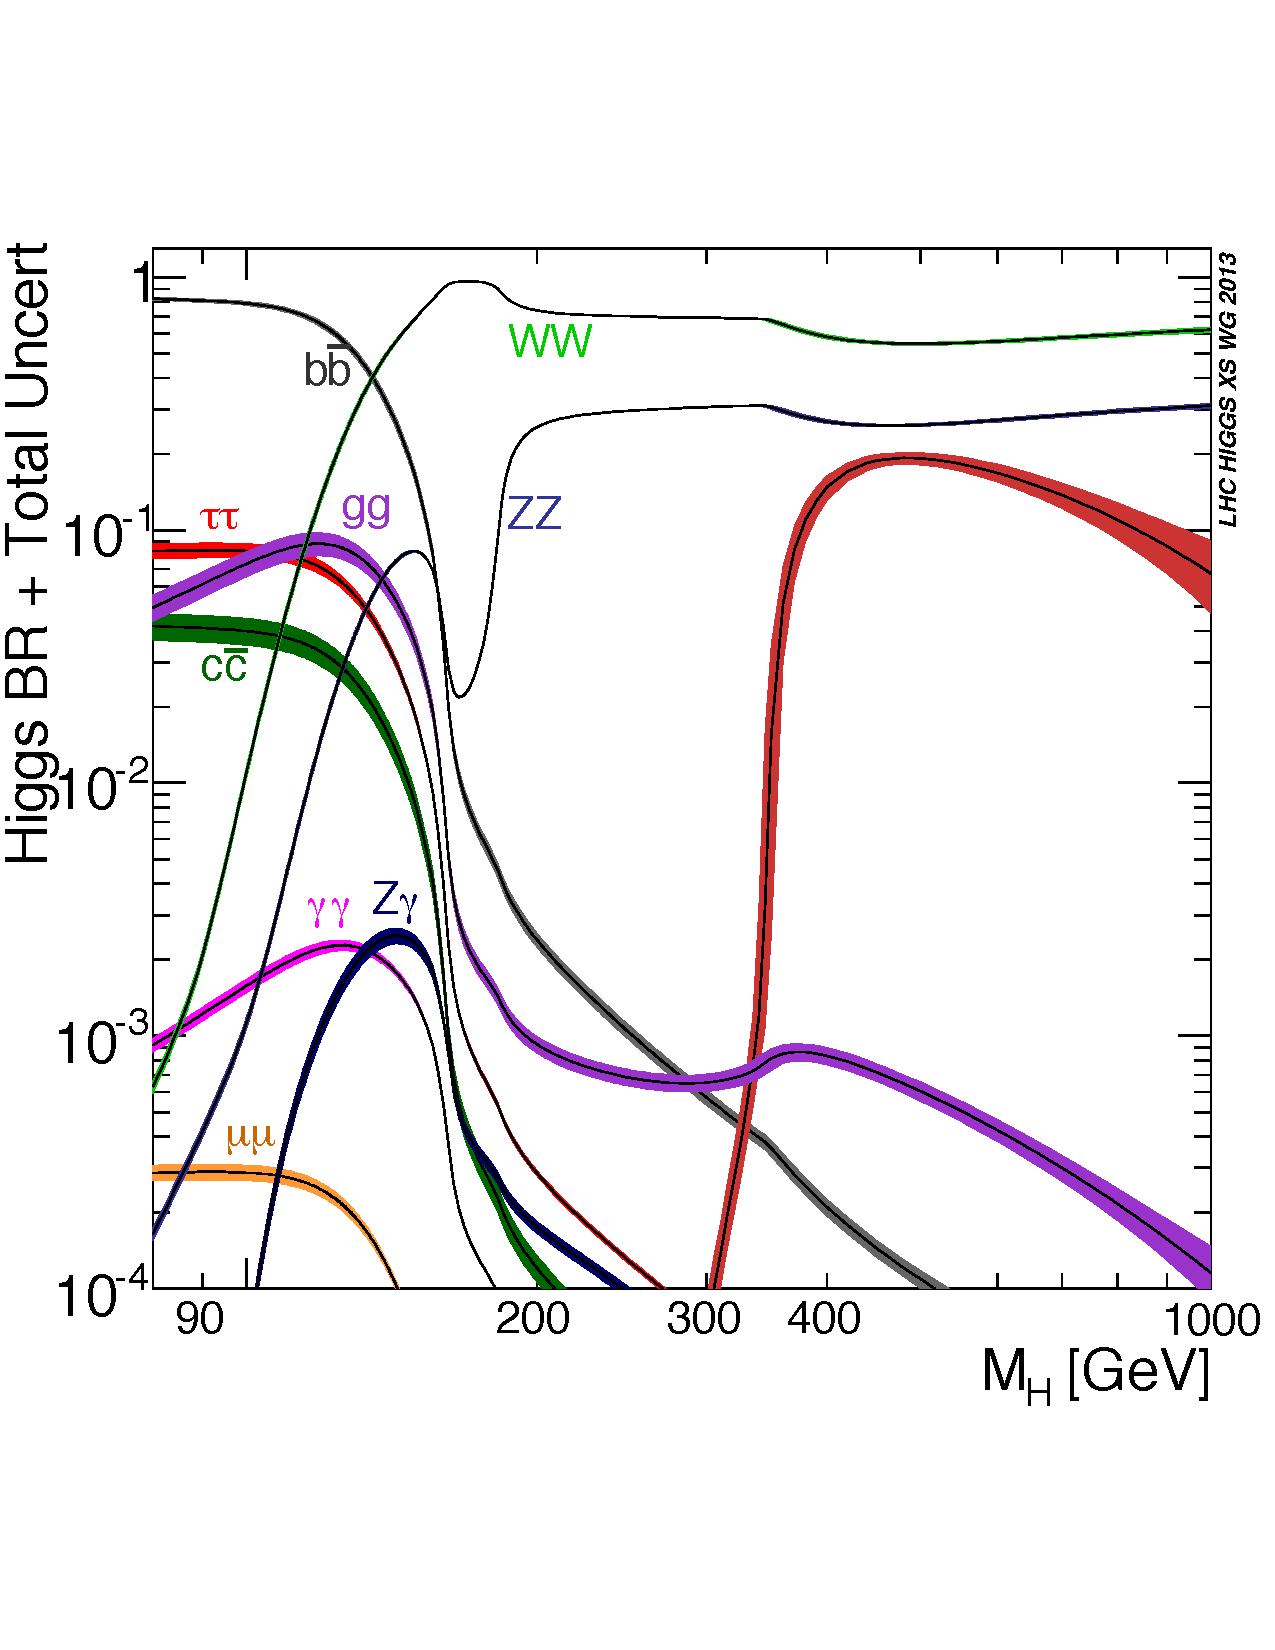
\includegraphics[width=0.45\linewidth]{{LHC_Pheno/Higgs_BR}.pdf}
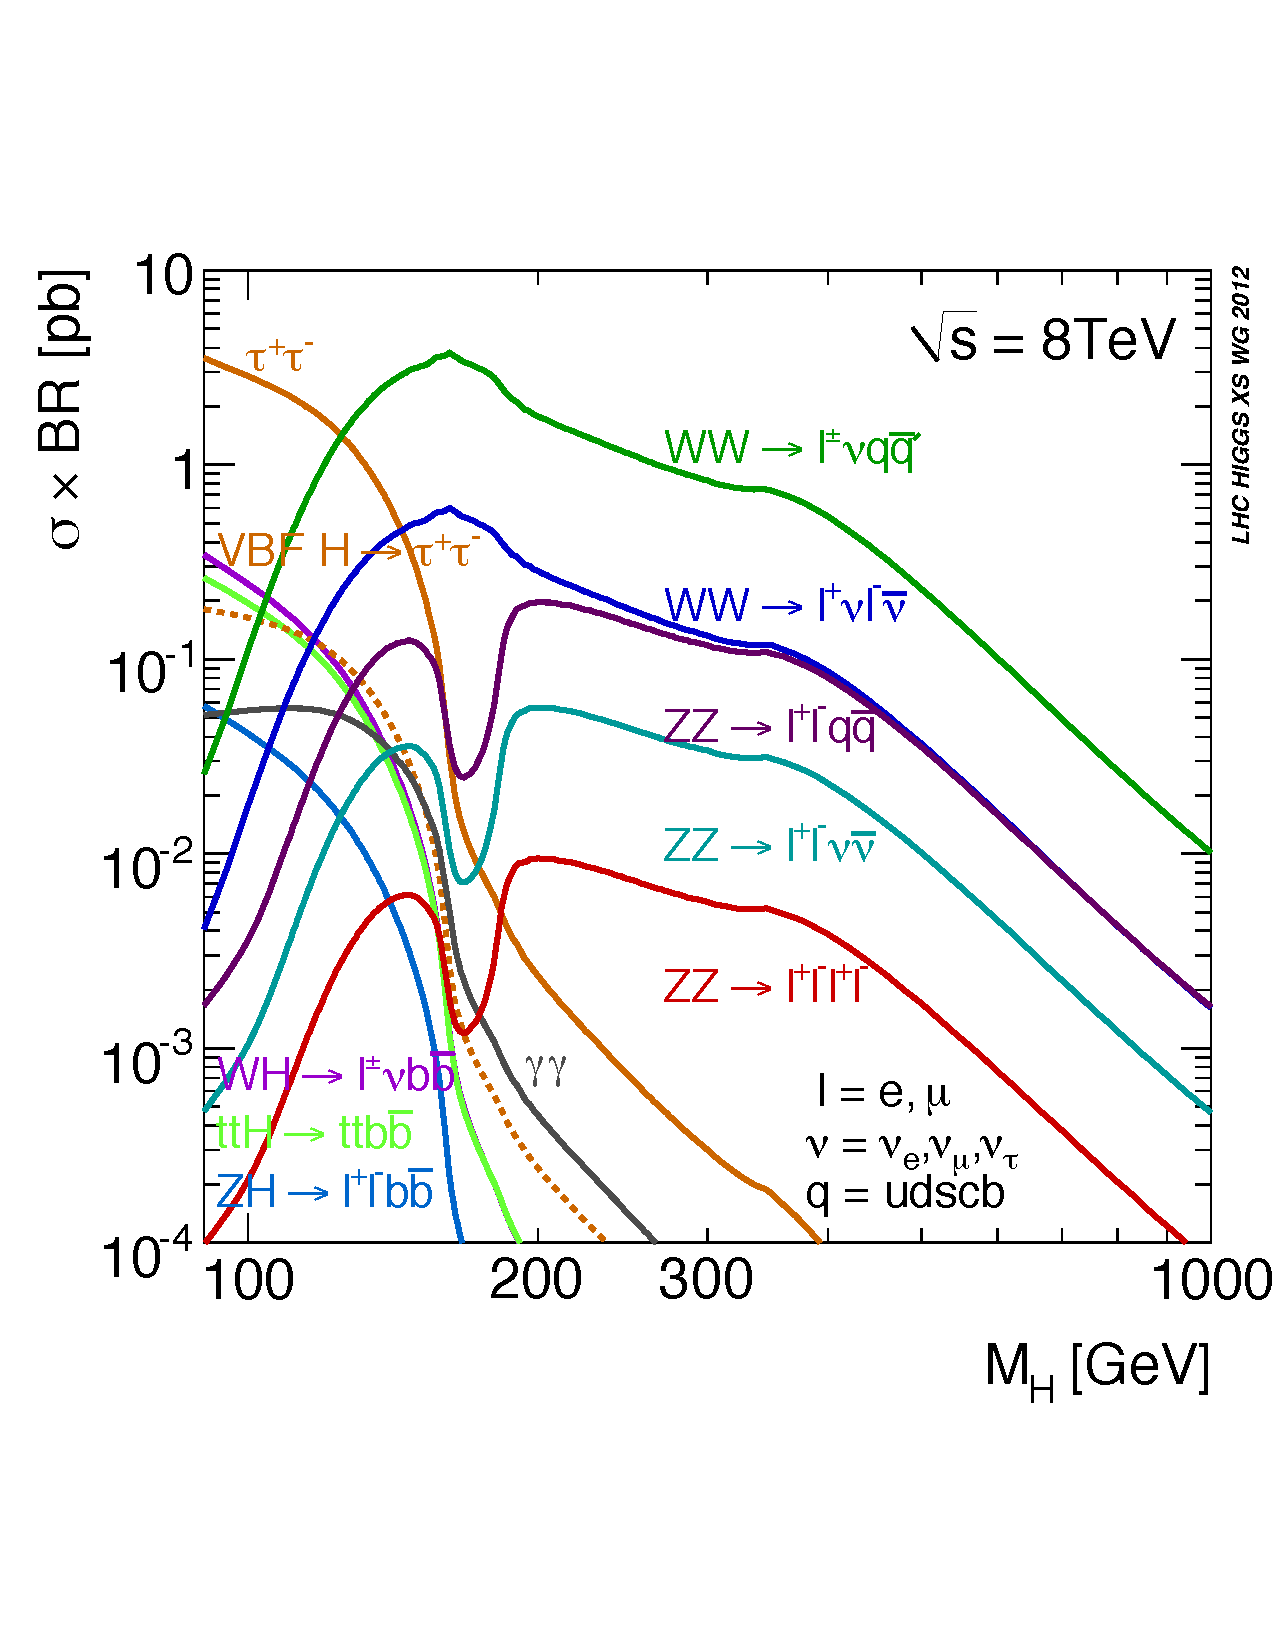
\includegraphics[width=0.46\linewidth]{{LHC_Pheno/XSBR_8TeV_SM_HM}.pdf}
\caption[(left) Standard Model Higgs boson decay branching ratios for selected decay modes, of specific interest for this thesis is the $ZZ$ branching ratio. (right) Branching ratio times cross section for selected final states, of specific interest for this thesis is the $ZZ \to 4\ell\left(\ell^{+}\ell^{-}\ell^{+}\ell^{-}\right)$.]{(left) Standard Model Higgs boson decay branching ratios for selected decay modes, of specific interest for this thesis is the $ZZ$ branching ratio. (right) Branching ratio times cross section for selected final states, of specific interest for this thesis is the $ZZ \to 4\ell\left(\ell^{+}\ell^{-}\ell^{+}\ell^{-}\right)$\cite{Dittmaier:2012vm, Heinemeyer:2013tqa}.}
\label{fig:Higgs_BR}
\end{center}
\end{figure}

Of specific interest for this thesis is the Higgs boson decay to the $ZZ \to 4\ell$ final state, shown in figure \ref{fig:H_ZZ_4l_Feyn}. Where we consider $\ell = e, \mu$ because these leptons will be long lived enough to be detected directly by CMS. Making them distinct from tau leptons which often decay because of their high mass. The $ZZ$ branching ratio is one of the highest across a wide rage of possible Higgs boson masses, making it advantageous for search and characterization studies. The $4\ell$ final state is used not because it has a particularly high cross section times branching ratio (seen in figure \ref{fig:Higgs_BR} right), but because there are low SM background contributions and because all of the final particles are directly detected by the CMS detector.

\begin{figure}
\begin{center}
\unitlength=2mm
\begin{fmffile}{H_ZZ_4l_Feyn}
\begin{fmfgraph*}(40,30) 
  \fmfleft{i1} \fmfright{sp1,sp2,sp3,sp4}
  \fmf{scalar,label=$H$}{i1,v1} 
  \fmf{boson,label=$Z$}{v1,v2}
  \fmf{boson,label=$Z$}{v1,v3}
  \fmf{fermion,label=$e/\mu$}{sp1,v2,sp2}
  \fmf{fermion,label=$e/\mu$}{sp3,v3,sp4}
\end{fmfgraph*}

\end{fmffile}
\end{center}
\caption[Feynman diagram depicting Higgs boson decay into two Z bosons and subsequently into four leptons $H \to ZZ \to 4\ell$.]{Feynman diagram depicting Higgs boson decay into two Z bosons and subsequently into four leptons $H \to ZZ \to 4\ell$.}
\label{fig:H_ZZ_4l_Feyn}
\end{figure}

This thesis considers all of the data collected by CMS during run 1 of the LHC proton-proton collisions. This corresponds to an integrated luminosity of $\unit{5.1}{\invfemtobarn}$ collected at a center of mass energy of $\sqrt{s} = \unit{7}{\TeV}$ and $\unit{19.7}{\invfemtobarn}$ collected at $\sqrt{s} = \unit{8}{\TeV}$. The search for and later characterization of a Higgs boson requires that there be two pairs of same-flavor, opposite-charge, well-identified isolated leptons $\left(e^{+}e^{-}e^{+}e^{-}, \mu^{+}\mu^{-}\mu^{+}\mu^{-}, \text{ or } e^{+}e^{-}\mu^{+}\mu^{-}\right)$ compatible with an intermediate state of $ZZ$. Computability with $ZZ$ is defined such that one or both of the $Z$'s is can be off the mass resonance.

In this case, a Higgs boson signal will appear as a narrow mass peak on top of a smooth background when observing the four lepton mass distribution. The search is conducted in a mass range of $m_{4\ell} \in \unit{110 -- 1000}{\GeV}$. For low-mass Higgs bosons $\left(m_{H} < \unit{400}{\GeV}\right)$, the width of the resonance in $m_{4\ell}$ will be very well peaked and is described with a Breit-Wigner distribution. For higher mass Higgs bosons $\left(m_{H} > \unit{400}{\GeV}\right)$, the width of the $m_{4\ell}$ mass peak will be much broader and described in the complex pole scheme \cite{Dittmaier:2011ti, Dittmaier:2012vm, Heinemeyer:2013tqa}. Detailed analysis of the width of the Higgs will be discussed in section \ref{sec:Higgs_Width_Pheno}.



\section{Higgs off resonance production and decay}
\label{sec:Higgs_Width_Pheno}

\section{Spin and Parity of a Single-Produced Resonance}